\section{Analysis}\label{sec:analysis}

A number of parameters can be tweaked to change the patch matching and storage, and different choices may be appropriate for different applications and performance requirements (both quantitative and qualitative). These parameters include the size of the input images, the size and shape of the patches extracted, the extraction strategy (non-overlapping vs overlapping patches), the sampling strategy used to seed the dictionary, the similarity metric and thresholds used to compare patches, as well as the parameters required for indexing and retrieving patch matches (approximate nearest neighbors). Here we discuss some of the parameter choices made and the experiments that lead up to these choices. Other possible choices are discussed in Sec.\ref{sec:futureext}.

Our quantitative performance metrics involve examining how the patch dictionary size grows with the addition of new images to the database (the growth function and rate) and the compression ratio per image (viewed as a distribution over compression ratios and summarized as the average compression ratio). Qualitative evaluations involve determining whether a human can spot compression artifacts and how salient they are in the images. The authors of this paper manually examined images reconstructed from the dictionary patches. A crowdsourced evaluation strategy involving Amazon's Mechanical Turk may be appropriate for larger-scale studies, but was beyond the scope of this paper.

There will always be a trade-off between compression benefits (storage - patch dictionary size, speed - image reconstruction time) and reconstruction quality. For many computer vision tasks including scene recognition (and thus retrieval), imperfect reconstructions with artifacts may not be a problem as long as the overall scene structure does not change. For instance, \cite{tiny_images} has shown that with images of pixel dimension 32x32, humans are already able to achieve over $80\%$ scene and object recognition rate. See fig.\ref{fig:badrecon} for a demonstration of an image that has serious reconstruction artifacts, but when down sampled (to a thumbnail), they become insignificant, and thus do not necessarily impair visual recognition.

 \begin{figure}
%\hspace{-25mm}
\centering
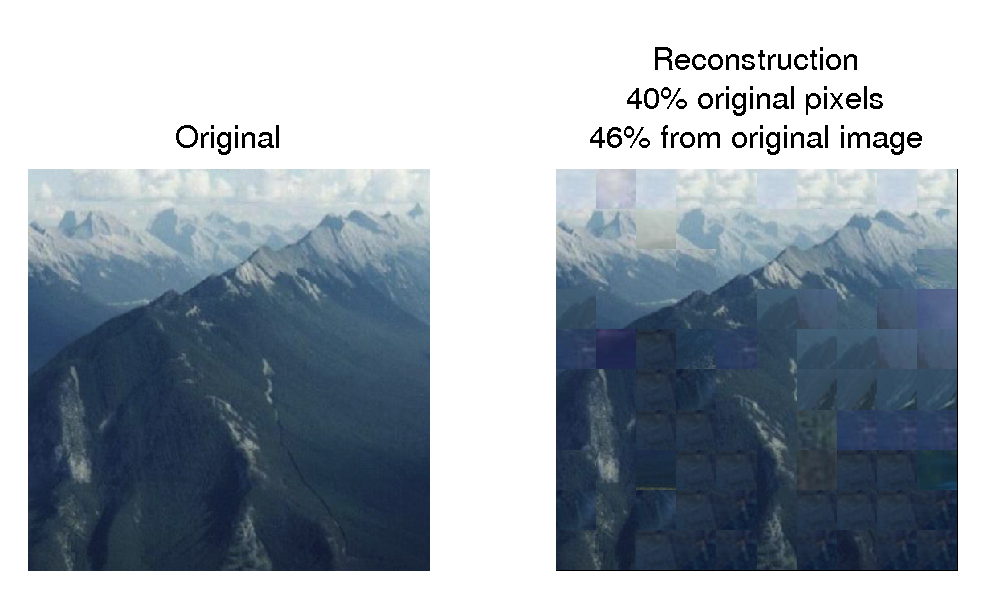
\includegraphics[width=1\linewidth]{Figures/184.png}
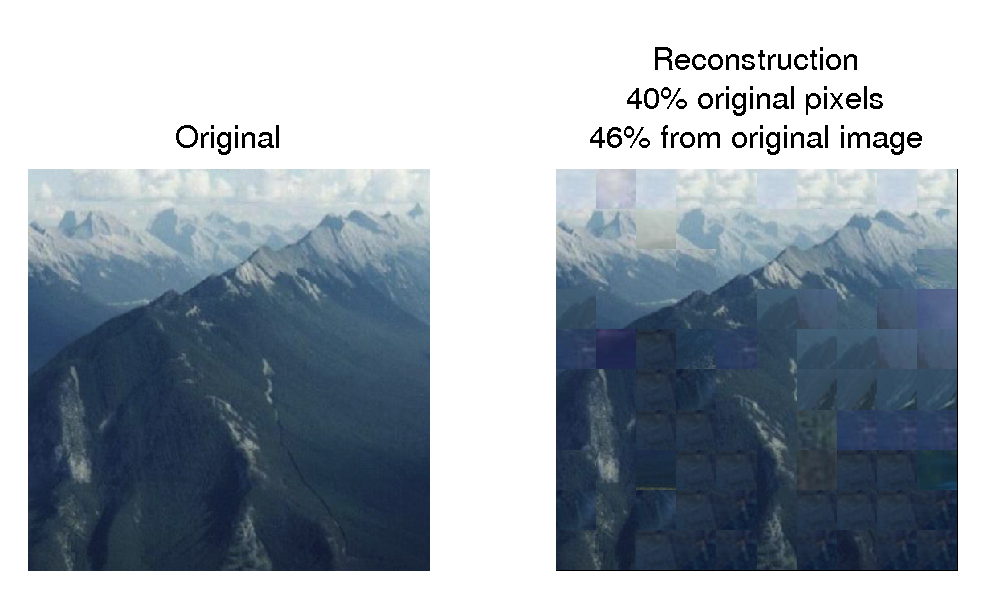
\includegraphics[width=0.5\linewidth]{Figures/184.png}
\caption{For demonstration purposes only, we choose a large patch size and low similarity threshold. Under these parameters, the original image is reconstructed to take up only $40\%$ of its original size (in pixels). The $60\%$ of the patches that have been replaced come either from the same image ($46\%$ of them), or from other images (the remaining $64\%$). Notice that when the size of the image and its reconstruction are halved, the artifacts already become visually insignificant, and would not impair a scene recognition or search task. }
\label{fig:badrecon}
\end{figure}


%\subsection{Quality Metrics}\label{ssec:qual-met}
%There are many possible formulations of these quality constraints; we detail those that we considered for this paper in section TODO.  Beyond mathematical metrics, subjective methods are also interesting to consider for formulating the quality constraints; one could imagine a scenario in which image quality is assessed by humans through a crowdsourced system, perhaps using an engine such as Amazon's Mechanical Turk TODO: cite.  We consider such subjective similarity metrics outside the scope of this paper and focus on the mathematical metrics for now.

%We wish to construct a database that trades off minimizing the amount of required space with maximizing read and write speeds of the data.

\subsection{Patch Size}

TODO(Zoya,Andrew): tradeoffs for patch size

Assume for now that we choose to store $p$ patches in our auxiliary table.  In practice, we choose $p$ to be a function $p \colon Function \to \mathds{N}$ which maps from our similarity metric to a number of patches to store.  Assume also that each patch is square and composed of $n^2$ pixels, where $n$ is a user defined parameter.  We further assume that each pixel requires 8 bytes to store  and that each pointer is 8 bytes (a standard integer for a 64-bit system).  Under this "image only" scheme, in the case where we have $i$ images, the cost $c_i$ to store all the images in our database is:

\begin{equation}
	c_i(i, m) = 8  i  m^2
\end{equation}

In the case where we store pointers to patches, we have two tables: one table to store pointers to image patch exemplars, and a second table to store the exemplar data themselves.  Under this "patch pointer"scheme, in the case where we have $i$ images and $p$ patches, the cost $c_p$ to store all the images in our database is:

\begin{equation}
	c_p(i, p, m, n) = 8 i (\frac{m}{n})^2 + 8  p  n^2
\end{equation}.

The first term is the cost of storing the pointer data, while the second term is the cost of storing the patch exemplars themselves.


\subsection{Sampling strategies}

A patch dictionary can be built up incrementally, adding new patches as new images are added to the database. A potential problem with this approach is that image reconstruction quality will tend to decrease with the order in which images are added, such that images added to the database earlier will tend to have more patches that correspond to them (see Fig.\ref{fig:sampStrategy} for an example). A strategy with a more even distribution of reconstruction quality over images involves starting with a batch of images, and seeding the dictionary by randomly sampling patches from a set of images from the batch. This is the strategy we employ. 

 \begin{figure}
%\hspace{-25mm}
%\centering
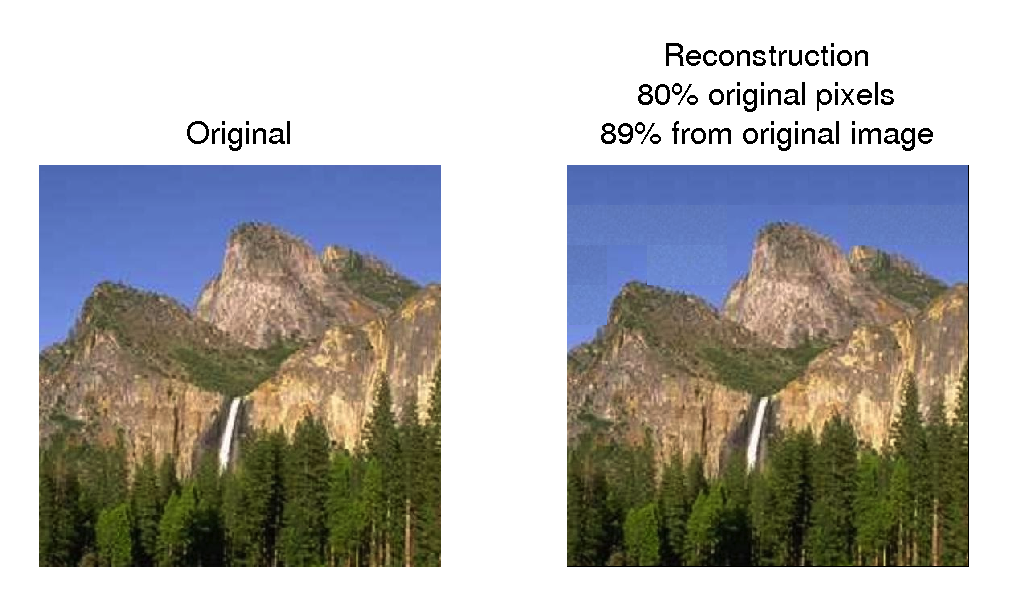
\includegraphics[width=1\linewidth]{Figures/009.png}
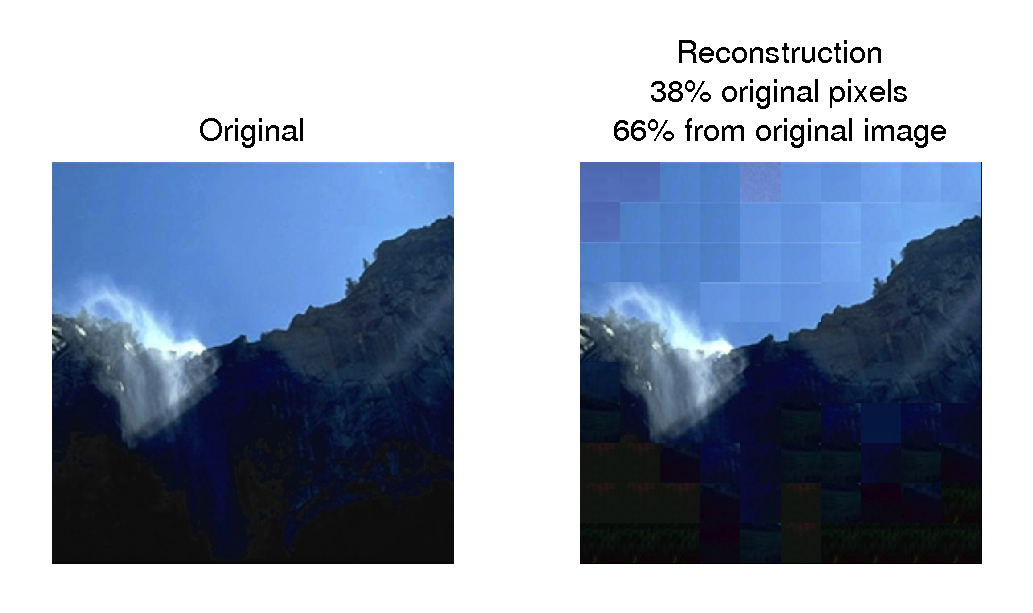
\includegraphics[width=1\linewidth]{Figures/014.png}
\caption{Example of a biased patch dictionary construction strategy, leading to non-uniformity in image reconstruction quality. Images added to the database earlier (top row) are better reconstructed (due to more patch samples in the database) than images added later (bottom row), constrained to be constructed out of patches added initially. The sky pixels in the image added later are borrowed from sky pixels of other images ($44\%$ of the pixels in this image come from other images, compared to only $11\%$ in the image on the first row). Note: here we use a very low patch similarity threshold and large patch size for demonstration purposes only, to emphasize the artifacts created.}
\label{fig:sampStrategy}
\end{figure}


\subsection{Similarity Threshold}

Many image (more specifically, patch) similarity functions are possible, each with its own distinct set of parameters that can be tweaked for the required application. Because we are dealing with patches of a size specifically chosen to increase within-patch homogeneity, we do not consider cases of patches containing objects (the most we expect is an object boundary or simple texture), and thus do not need to consider complex image similarity functions (like SIFT matching, spatial relationship-preserving functions, etc.). We can constrain ourselves to color similarity, where a patch is a collection of pixels, each of which is defined to be a triplet of integer values, assuming a 3-D color space.

\begin{displaymath}
S(P_1, P_2) = \frac{||p_1 - p_2||^2}{n^2}
\end{displaymath}

Figure \ref{fig:colProblem} demonstrates what happens when we do not separately constrain each of the color channels to match. We have patches that match in terms of general hue (average of the color channels), but are the wrong color and produce visible visual artifacts.

 \begin{figure}
%\hspace{-25mm}
%\centering
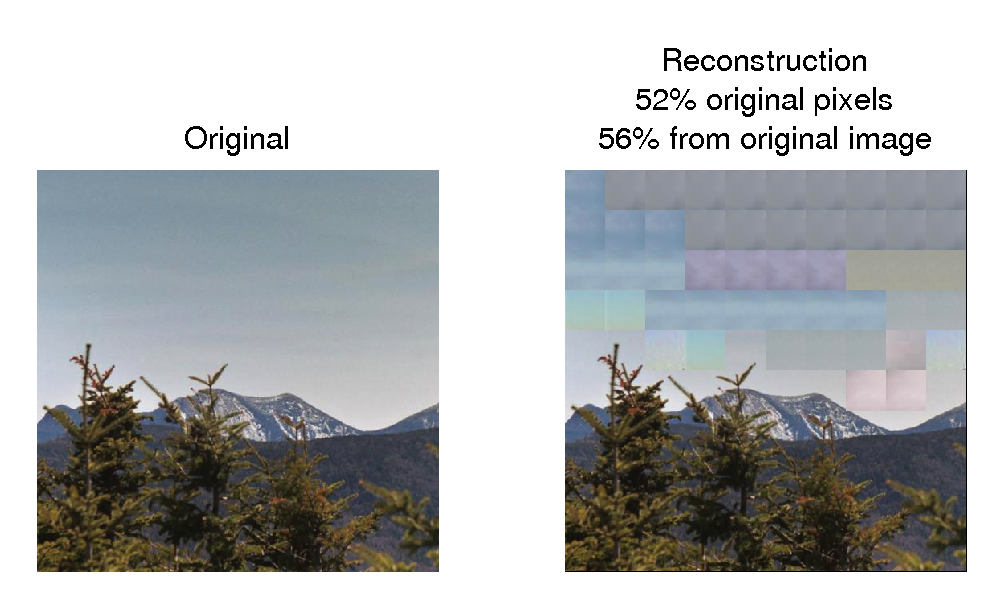
\includegraphics[width=1\linewidth]{Figures/197.png}
\caption{}
\label{fig:colProblem}
\end{figure}

